\chapter{Launch and manage instances}\label{cha:launch-manage-inst}
Instances are virtual machines that run inside the cloud. You can launch
an \gls{instance} from the following sources:

\begin{itemize}
\item Images uploaded to the Image service.  Note that, because images
  are read-only, any changes made while the instance is running will
  be lost when the instance is deleted, unless you choose to ``Create
  New Volume''.  If you create a new volume, the VM's state will
  persist on the volume, even when the current instance is deleted.
  \item Image that you have copied to a persistent volume. The instance
  launches from the volume, which is provided by the
  \textbf{cinder-volume} API through iSCSI.
\item Instance snapshot that you took.
\end{itemize}

\section{Launch an instance}\label{launch-an-instance}
\begin{enumerate}
\item Open the Compute tab and select the Instances category.

  The dashboard shows the list of existing instances with their name,
  IP addresses, flavor, status, power state, \ldots
\item Click \strong{Launch Instance}.
\item In the Launch Instance dialog box, specify the following values:

  \begin{center}
    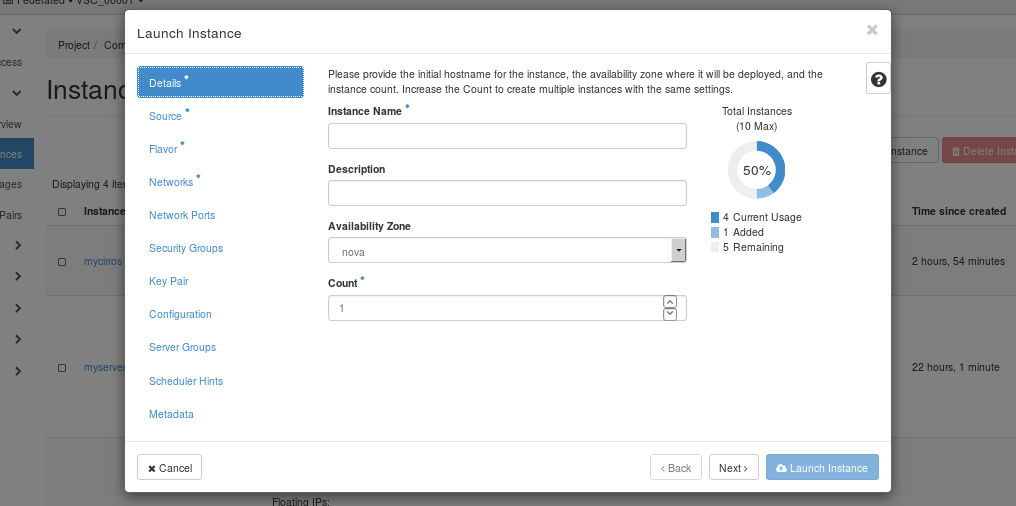
\includegraphics[scale=0.5]{img/tab-compute-instances-launch.png}
  \end{center}
  
  \begin{description}
  \item[Details] tab
    \begin{description}
    \item[Instance Name] Assign a name to the virtual machine.

      \strong{Note:} The name you assign here becomes the initial host
      name of the server. If the name is longer than 63 characters,
      the Compute service truncates it automatically to ensure dnsmasq
      works correctly.

      After the server is built, if you change the server name in the
      API or change the host name directly, the names are not updated
      in the dashboard.

      Server names are not guaranteed to be unique when created so you
      could have two instances with the same host name.

    \item[Description] You can assign a brief description of the
      virtual machine.
    \item[Availability Zone] By default, this value is set to the
      availability zone given by the cloud provider (for example,
      \strong{us-west} or \strong{apac-south}).  For some cases, it
      could be \strong{nova}.
    \item[Count] To launch multiple instances, enter a value greater
      than \strong{1}. The default is \strong{1}.
    \end{description}

    \begin{center}
      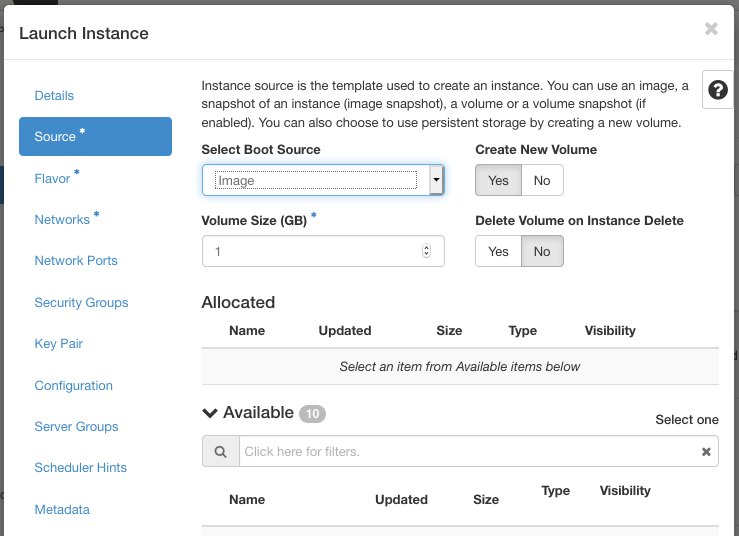
\includegraphics[width=0.7\textwidth]{img/launch_instance_source}
    \end{center}
  \item[Source] tab
  \begin{description}
  \item[Select Boot Source] Your options are:
    \begin{description}
    \item[Image]
    \item[Image snapshot]
    \item[Volume]
    \item[Volume snapshot]
    \end{description}
    Depending on the type of boot source, the list of available items
    changes.

  \item[Create New Volume] If you enable this option when launching
    from an image or instance snapshot, the image or snapshot will be
    copied to a volume.  This way, the state of your instance persists
    after shutdown and reboot.
  \end{description}

\item[Flavor] tab. Specify the size of the instance to launch.

  \strong{Note:} The flavor is selected based on the size of the image
  selected for launching an instance. For example, while creating an
  image, if you have entered the value in the Minimum RAM (MB) field
  as 2048, then on selecting the image, the default flavor is
  \textbf{m1.small}.  If a `!' warning sign is displayed next to a
  resource for one of the flavors, that means that this flavor would
  exceed the project's quota for that resource, and therefore is not
  available.

\item[Networks] tab. Add one or more networks to the instance.

\item[Network Ports] tab. Activate the ports that you want to assign to
  the instance.
\item[Security Groups] tab. Activate the security groups that you want
  to assign to the instance.

  Security groups are a kind of cloud firewall that define which
  incoming network traffic is forwarded to instances.  See section
  \ref{cha:conf-access-secur} on page ~\pageref{sec:security-groups}
  for more information.

  The default security group is assigned to the instance
  automatically.
\item[Key Pair] tab. Specify a key pair.

  If the image uses a static root password or a static key set
  (neither is recommended), you do not need to provide a key pair to
  launch the instance.
\item[Configuration] tab. Specify a customization script that runs
  after your instance launches.

\item[Server Groups] tab.

\item[Scheduler Hints] tab.

\item[Metadata] tab. Add Metadata items to your instance.
\end{description}

\item Click \strong{Launch Instance}.
\end{enumerate}

The instance starts on a compute node in the cloud.

\strong{Note:} If you did not provide a key pair, security groups, or
rules, users can access the instance only from inside the cloud
through VNC. Even pinging the instance is not possible without an ICMP
rule configured.

You can also launch an instance from the Images or Volumes category when
you launch an instance from an image or a volume respectively.

When you launch an instance from an image, OpenStack creates a local
copy of the image on the compute node where the instance starts.

For details on creating images, see
\href{https://docs.openstack.org/image-guide/create-images-manually.html}{\emph{Creating
images manually}} in the \emph{OpenStack Virtual Machine Image Guide}.

\section{Connect to an instance using SSH}\label{connect-to-your-instance-using-ssh}
Before you can connect to an instance using SSH, you must set up a
floating IP, as discussed in section~\ref{sec:floating-ip}.

You can only reach the floating IP's from the UGent login node
\lstinline{login.hpc.ugent.be}, so you'll need to access the UGent
login node first, and hop to your instance from there.  If you do not
have a suitable private key in your VSC storage space, you need to set
up an SSH agent with key forwarding locally, i.e.\ on the machine
where you store the private key of an authorized keypair for the
instance.  Section 2.1.4 of the HPC tutorial explains how to set this
up (\url{https://www.vscentrum.be/support/tut-book/vsc-tutorials}).

\begin{enumerate}
\item Connect to the UGent login node, using the \lstinline{ssh -A} option
  to enable agent forwarding:

  \begin{prompt}
    %\shellcmd{ssh -A vsc12345@login.hpc.ugent.be}
  \end{prompt}

\item Copy the address of the floating IP where your instance can be
  reached.  In our example, the address is 193.190.85.40.

\item From the login node, connect to the instance.  Use OpenSSH's
  \lstinline{-p} option to specify the port where the instance's SSH
  server can be reached, e.g. for port 50022:

  \begin{prompt}
    %\shellcmd{ssh -p 50022 ubuntu@193.190.85.40}
  \end{prompt}

  The default images do not allow SSH logins for the root user.  There
  is a default user instead, who can get administrative privileges
  using \lstinline{sudo}.  In our example, we have used the username
  \lstinline{ubuntu} for Ubuntu images.  Attempting to log in as root
  will return an error message with the proper user name.
\end{enumerate}

\section{Track usage for instances}\label{track-usage-for-instances}

You can track usage for instances for each project. You can track costs
per month by showing meters like number of vCPUs, disks, RAM, and uptime
for all your instances.

\begin{enumerate}
\item Open the Compute tab and select the Overview category.
\item To query the instance usage for a period of time, select a time
  range and click \strong{Submit}.
\item To download a summary, click \strong{Download CSV Summary}.
\end{enumerate}

\section{Create an instance snapshot}\label{create-an-instance-snapshot}

\begin{enumerate}
\item Open the Compute tab and select the Instances category.
\item Select the instance from which to create a snapshot.
\item In the actions column, click \strong{Create Snapshot}.
\item In the Create Snapshot dialog box, enter a name for the snapshot, and
  click \strong{Create Snapshot}.
\end{enumerate}

The Images category shows the instance snapshot.

To launch an instance from the snapshot, select the snapshot and click
Launch. Proceed with launching an instance.

\section{Manage an instance}\label{manage-an-instance}

\begin{enumerate}
\item Open the Compute tab and select the Instances category.
\item Select an instance.
\item In the menu list in the actions column, select the state.

  You can resize or rebuild an instance. You can also choose to view
  the instance console log, edit instance or the security
  groups. Depending on the current state of the instance, you can
  pause, resume, suspend, soft or hard reboot, or terminate it.
\end{enumerate}

\subsection*{Difference between \emph{suspend}, \emph{pause}, \emph{shelve}, \emph{shut off}, \emph{delete}}\label{server-power-down-states}

\begin{description}
\item[Pause] Stores the state of the VM in the (RAM) memory.
\item[Suspend] Stores the state of the VM on the disk, all memory is
  written to disk, and the server is stopped.
\item[Shut off] The server is powered down by the user, either through
  the OpenStack Compute API, or from within the server by issuing a
  \emph{shutdown -h} command. In this state the user retains all
  computational resources associated with the VM. The instance can be
  later restarted.
\item[Shelve] Shelving stops the instance and takes a snapshot of
  it. Then depending on the value of the \emph{shelved\_offload\_time}
  config option, the instance is either deleted from the hypervisor
  (0), never deleted (-1), or deleted after some period of time (>
  0). Shelve preserves all associated data and VM resources but does
  not retain anything in memory.
\item[Delete] The VM is deleted and removed from \gls{OpenStack}
  together with any associated processes and resources.  However, for
  instances backed by a persistent volume, this volume is not deleted.
  When such an instance is deleted, you can restore it by launching a
  new instance from the volume, or delete the volume as well (see
  section \ref{delete-a-volume}).
\end{description}

For more details see the OpenStack documentation on \href{https://docs.openstack.org/nova/\osversion/reference/vm-states.html}{\emph{Virtual Machine States and Transitions}} and \href{https://developer.openstack.org/api-guide/compute/server_concepts.html}{\emph{Server concepts}}.

%%% Local Variables:
%%% mode: latex
%%% TeX-master: "intro-Cloud"
%%% End:
